En este capítulo se describirá el modelo en el cual se basa toda la investigación, también se definirán los conceptos utilizados a lo largo del trabajo como la definición de la presión social y los blocking clusters. Además se comentará el algoritmo de Verlet, ya que fue utilizado para resolver la dinámica del problema. 

\section{\label{sfm}Modelo de Fuerza social}

El modelo de fuerza social es un modelo basado en agentes utilizado para simular el movimiento de peatones. Supone que los individuos soportan tres tipos de fuerzas: fuerzas de deseo (autopropulsión), sociales (repulsión) y granulares (rozamiento).  \\

La fuerza de autopropulsión refleja el hecho que el individuo i-esimo que posee masa $m_i$, desea  moverse con una velocidad $v_d^ {(i)}(t)$ en una dirección $\hat{\mathbf{e}}_d^ {(i)}(t)$, por lo tanto readapta su velocidad $\mathbf{v}_i(t)$ con un cierto tiempo característico $\tau$.
\begin{equation}
\mathbf{f}_d^ {(i)}(t)=m_i\,\displaystyle\frac{v_d^ {(i)}(t)\,\hat{\mathbf{e}}_d^ {(i)}(t)-\mathbf{v}_i(t)}{\tau}\label{fdeseo}
\end{equation}

La repulsión social es una fuerza que describe la tendencia que tienen las personas a mantenerse alejadas unas de otras. Depende de la distancia de separación entre individuos $d_{ij}=\left\|\mathbf{r_i}-\mathbf{r_j}\right\|$ y está en la dirección normal $\mathbf{n}_{ij}=(n_{ij}^1,n_{ij}^2)/d_{ij}$ (versor que apunta desde el individuo j al individuo i). Los peatones están en contacto si el valor de $d_{ij}$ es más chico que la suma de los radios $r_{ij}=(r_i+r_j)$. $A_i$ y 	$B_i$ son constantes.

\begin{equation}
\mathbf{f}_s^{(ij)}=A_i\,e^{(r_{ij}-d_{ij})/B_i}\mathbf{n}_{ij}\label{fsocial}
\end{equation} 

Cuando los individuos están en contacto, comienza a actuar una fuerza de rozamiento, la misma es proporcional a la velocidad relativa entre los mismos.  
$\Delta \mathbf{v}_{ij}=(\mathbf{v}_i-\mathbf{v}_j)$, la dirección tangencial está representada por $\mathbf{t}_{ij}=(-n_{ij}^2,n_{ij}^1)$.  $\kappa$ es una constante y $g(x)$ es una función nula cuando los individuos no se tocan $(r_{ij}<d_{ij})$ y toma el valor de su argumento en caso contrario. 
\begin{equation}
\mathbf{f}_g^{(ij)}=\kappa\,g(r_{ij}-d_{ij})\,\Delta \mathbf{v}_{ij}\cdot\mathbf{t}_{ij}\label{frozamiento}
\end{equation}

Se trata de forma análoga a la interacción de los individuos con las paredes. $d_{iW}$ es la distancia del i-esimo peatón con la pared W, $n_{iW}$ la dirección perpendicular entre éstos y $t_{iW}$ la tangencial. La expresión \ref{fparedes} agrupa tanto a la repulsión como al rozamiento de la interacción peatón-pared.

\begin{equation}
\mathbf{f}^{iW}=A_ie^{(r_{i}-d_{iW})/B_i}\mathbf{n}_{iW}-\kappa g(r_{i}-d_{iW})\Delta \mathbf{v}_{i}\cdot\mathbf{t}_{iW}
\label{fparedes}
\end{equation} 

Con todo esto, mediante la fórmula \ref{newton}, puede expresarse la variación de velocidad en el tiempo que siente un individuo. $f^{ij}$ es el término de interacción entre individuos, es la suma de la repulsión y el rozamiento. El cambio de posición viene dado por $v_{i}(t)=d\mathbf{r_i}/dt$.

\begin{equation}
m_i\frac{d\mathbf{v_i}}{dt}=\mathbf{f}_d^ {(i)}(t)+ \sum_{i\neq j}^{N}\mathbf{f}^{(ij)} + \sum_{W}^{N}\mathbf{f}^{(iW)}
\label{newton}
\end{equation}  

Uno de los resultados más trascendentes de este modelo es el efecto "Faster is slower" \cite{Helbing1}. A partir de cierto grado de apuro ($v_d=2$~m/s) un incremento en la velocidad de deseo produce evacuaciones menos eficientes (los peatones tardan más en evacuar). 
 
\section{Presión local}

A pesar de que la fuerza de deseo $\mathbf{f}_d$ y la fuerza social $\mathbf{f}_s$, del modelo de fuerza social, no son magnitudes "Físicas" (\textit{i.e.} no tienen par de reacción), la ecuación de movimiento sigue siendo válida. Por lo tanto, se puede derivar la relación del virial\cite{lion}. 

\begin{equation}
 \bigg\langle\displaystyle\sum_{i=1}^N\displaystyle\frac{p_i^2}{m_i} + 
\displaystyle\sum_{i=1}^N 
\mathbf{r}_i\cdot\mathbf{f}_i\bigg\rangle=0\label{virial1}
\end{equation}


\noindent Para un conjunto de $N$ pedestrians. $p_i$  y $\mathbf{f}_i$ son el impulso y la fuerza total actuando sobre el individuo $i$. $\langle\cdot\rangle$ corresponde al valor medio en el tiempo.  \\

La presión local para un peatón ($i$) está asociada a las fuerzas (por unidad de área) actuando sobre él debidas a los individuos que lo rodean y las paredes. Según Ref.~\cite{lion} se puede definir la "función de presión social" $P_i$ como:\\

\begin{equation}
3P_iV_i=\displaystyle\frac{p_i^2}{m_i} + \frac{1}{2}
\displaystyle\sum_{j=1}^{N-1}
\mathbf{r}_{ij}\cdot\mathbf{f}_s^{(ij)}\label{pv}
\end{equation}

\noindent donde $V_i$ es el volumen que encierra al peatón $i$ y 
$\mathbf{r}_{ij}=\mathbf{r}_{i}-\mathbf{r}_j$. Cabe destacar que el producto interno $\mathbf{r}_{ij}\cdot\mathbf{f}_s^{(ij)}$ siempre es positivo debido a la repulsión y es igual al producto escalar $d_{ij}f_s^{(ij)}$.  \\ 

El segundo término en la equación \ref{virial1} puede dividirse en la suma de productos internos $\mathbf{r}_i\cdot\mathbf{f}_d$ (deseo), 
$\mathbf{r}_i\cdot\mathbf{f}_s$ (social) y $\mathbf{r}_i\cdot\mathbf{f}_g$ (granular). De hecho, la suma del producto social depende de la distancia entre partículas $d_{ij}f_s^{(ij)}$, mientras que la parte granular no tiene ningún rol por su ortogonalidad ($\mathbf{r}_{ij}\cdot\mathbf{f}_g^{(ij)}=0$). Por lo tanto, la relación del virial (\ref{virial1}) se expresa \\  


\begin{equation}
 \displaystyle\sum_{i=1}^N\langle3P_iV_i 
\rangle=-\displaystyle\sum_{i=1}^N \langle
\mathbf{r}_i\cdot\mathbf{f}_d^{(i)}\rangle\label{virial2}
\end{equation}

Hay que destacar que la ecuación (\ref{virial2}) se cumple si los peatones están en contacto o no. La "función de presión social" $P_i$ hace que los individuos puedan cambiar su patrón de comportamiento cuando se acercan mucho unos con otros o con las paredes. \\ 


\section{Blocking Clusters}

Se utilizó el concepto de blocking cluster~\cite{Dorso1} para estudiar a los individuos más cercanos a la salida. Se lo define como un conjunto de individuos en contacto que va desde un punto de la pared hacia otro. Estos puntos están próximos a los costados de la puerta. Aquellos peatones que conforman el blocking cluster son los responsables de bloquear la salida. Típicamente los blocking cluster formados en las evacuaciones tiene estructura de "arco" como el que se muestra en la figura \ref{bc}. Basta que un solo peatón deje de estar en contacto con sus vecinos para que el blocking cluster deje de estar constituído. \\

\begin{figure}[H]
    \centering
    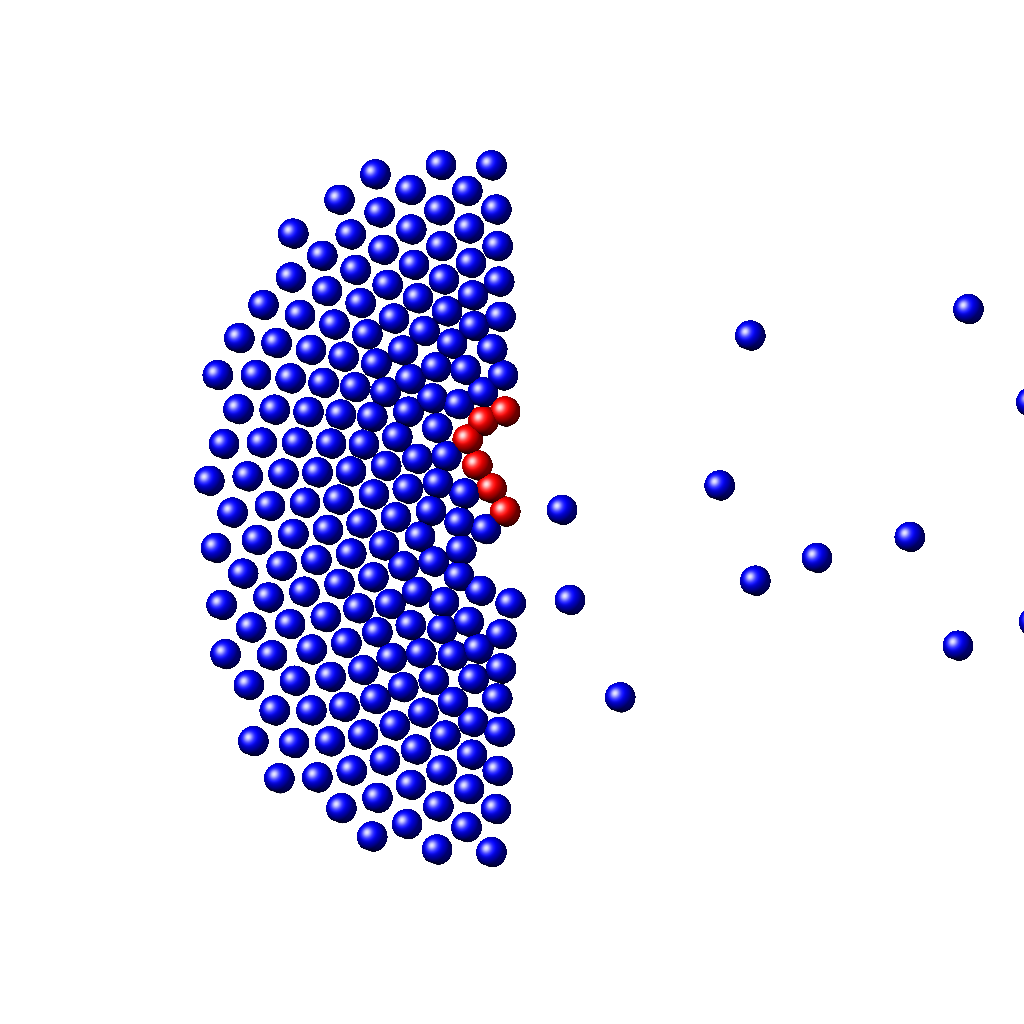
\includegraphics[height=5.5cm]{figuras/in_image_2_120000_bkg.png}
    \caption[width=5cm]{}
    \label{bc}
\end{figure}

A lo largo del trabajo se han usado dos tipos de blocking clusters: Big blocking cluster y small blocking cluster. El primero se tiene cuando hay dos puertas sobre la misma pared, son los individuos que van desde una puerta hasta la otra (encierran las dos salidas). El segundo es el bloqueo de una única salida. 

\section{Algoritmo de Verlet}

Para integrar las ecuaciones de movimiento se usó el algoritmo de Verlet, este método es ampliamente utilizado en el campo de dinámica molecular.\\
Este algoritmo es una combinación de dos expansiones de taylor sumadas para dar lugar a una expresión con términos pares únicamente~\cite{haile}

\begin{equation}
x(t+\Delta t)=2x(t)-x(t-\Delta t)+\frac{d^2x(t)}{dt^2} \Delta t^2+O(\Delta t^4)
\label{verlet_x}
\end{equation} 
Este es el algoritmo de Verlet para posiciones. Tiene un error de truncamiento local de ($\Delta^4$), por lo tanto es de tercer orden aunque no contenga derivadas de tercer orden. La aceleración es obtenida de fuerzas intermoleculares y la segunda ley de Newton.
Para estimar la velocidad se utiliza:
\begin{equation}
v(t)\simeq \frac{x(t+\Delta t)-x(t-\Delta t)}{2\Delta t}
\label{verlet_v}
\end{equation}
Para resolverlo se suelen llevar a cabo los siguientes pasos: se actualizan las velocidades, luego las posiciones, en tercer lugar las fuerzas y se vuelve a repetir el ciclo hasta completar las trayectorias. 
El algoritmo de Verlet posee buena estabilidad para pasos temporales moderadamente grandes.
